% !TEX TS-program = pdflatexmk

\documentclass[14pt]{beamer}
\usepackage{newtxtext,newtxmath}
\usepackage{microtype}
\usepackage[english]{babel}
\usepackage{hyperref}
\usepackage{graphicx}
\usepackage{listings}
\lstloadlanguages{Python}
\lstset{language=Python}
\lstset{%
basicstyle=\ttfamily\bfseries,
keywordstyle=\color{blue}, emph={self}, emphstyle={\color{blue}},
identifierstyle=,
commentstyle=\color{brown},
stringstyle=\color{green!50!black},
showstringspaces=false,
emphstyle={[2]\color{purple}},
}
\usepackage{tikz}
\usepackage{pgfplots}
\usepackage{forest}
\usetikzlibrary{calc}
\usetikzlibrary{shapes}
\usetikzlibrary{positioning}
\usetikzlibrary{arrows}
\usepackage{array}
\newcolumntype{L}[1]{>{\raggedright\let\newline\\\arraybackslash\hspace{0pt}}m{#1}}

\mode<presentation>{
\usetheme{Madrid}
\definecolor{uabgreen}{cmyk}{.89,.31,.78,.17}
\usecolortheme[named=uabgreen]{structure}
\setbeamertemplate{navigation symbols}{}
\setbeamertemplate{footline}[frame number]
\setbeamertemplate{section in toc}[square]
\setbeamertemplate{subsection in toc}[square]
\setbeamertemplate{items}[square]
\setbeamercovered{transparent=5}
}

\newcommand{\keyword}[1]{{\color{blue}#1}}
\newcommand{\cmnt}[1]{{\color{gray}#1}}
\newcommand{\str}[1]{{\color{green!50!black}#1}}
\newcommand{\num}[1]{{\color{green!55!blue}#1}}
\newcommand{\defn}[1]{{\color{purple}#1}}

\newcommand{\limpl}{\Rightarrow}
\newcommand{\liff}{\Leftrightarrow}

\newcommand{\tab}{\hspace{1em}}

\author[Dr. Bethard]{Dr. Steven Bethard}
\institute[UAB CIS]{%
Computer and Information Sciences\\
University of Alabama at Birmingham}

\AtBeginSection[]
{
  \begin{frame}<beamer>{Outline}
    \tableofcontents[currentsection]
  \end{frame}
}

\tikzset{
  invisible/.style={opacity=0,text opacity=0},
  text visible on/.code={%
    \alt<#1>{}{\pgfkeysalso{text opacity=0}}
  },
  visible on/.code={%
    \alt<#1>{}{\pgfkeysalso{invisible}}
  },
  filled on/.code={%
    \alt<#1>{\pgfkeysalso{fill=gray}}{}
  },
  alt/.code n args={3}{%
    \alt<#1>{\pgfkeysalso{#2}}{\pgfkeysalso{#3}}
  },
}
\forestset{
  edge weight/.style={
    edge label={node[midway,above,sloped]{#1}}},
  invisible/.style={
    /tikz/invisible,
    edge={/tikz/invisible}},
  visible on filled on/.code n args={2}{%
    \alt<#1>{\alt<#2>{\pgfkeysalso{fill=gray}}{}}{\pgfkeysalso{invisible}}
  },
  visible on/.code={%
    \alt<#1>{}{\pgfkeysalso{invisible}}
  },
}

\newlength{\wumpusgridsize}
\newenvironment{wumpusgrid}[2]{%
\setlength{\wumpusgridsize}{#2}
\begin{tikzpicture}
\draw[very thick,step=\wumpusgridsize] (0,0) grid (#1\wumpusgridsize, #1\wumpusgridsize);
}{%
\end{tikzpicture}
}
\newcommand{\wumpustop}[5][]{%
\only<#2>{\node[#1] at (#3\wumpusgridsize+0.5\wumpusgridsize,#4\wumpusgridsize+0.75\wumpusgridsize) {#5};}
}
\newcommand{\wumpusbottom}[5][]{%
\only<#2>{\node[#1] at (#3\wumpusgridsize+0.5\wumpusgridsize,#4\wumpusgridsize+0.25\wumpusgridsize) {#5};}
}
\newcommand{\wumpusagent}[3]{\wumpusbottom{#1}{#2}{#3}{\fbox{A}}}
\newcommand{\wumpuspercept}[4]{%
\only<#1>{\node[red,inner sep=0pt] at (#2\wumpusgridsize+0.25\wumpusgridsize,#3\wumpusgridsize+0.75\wumpusgridsize) {\textbf{#4}};}
}
\newcommand{\wumpusknowledge}[4]{%
\only<#1>{\node[draw,cloud,inner sep=0pt,text width=1em,align=center] at (#2\wumpusgridsize+0.75\wumpusgridsize,#3\wumpusgridsize+0.75\wumpusgridsize) {\footnotesize #4};}
}

\lstset{emph={[2]__init__,__str__}}

\tikzset{
  red edge on/.code={%
    \only<#1>{\pgfkeysalso{draw=red,ultra thick}}
  },
  red fill on/.code={%
    \only<#1>{\pgfkeysalso{fill=red!25!white}}
  },
  red edge fill on/.code={%
    \only<#1>{\pgfkeysalso{draw=red,ultra thick,fill=red!25!white}}
  },
  blue edge on/.code={%
    \only<#1>{\pgfkeysalso{draw=blue,ultra thick}}
  },
  blue fill on/.code={%
    \only<#1>{\pgfkeysalso{fill=blue!25!white}}
  },
}


\title{Logical Agents}
\date{11 Feb 2014}

\begin{document}

\begin{frame}
  \titlepage
\end{frame}


\begin{frame}{Outline}
  \tableofcontents
\end{frame}


\section{Logical Agents}

\begin{frame}{Knowledge Bases}
\begin{block}{Idea: Separate Knowledge from Reasoning}
\begin{description}[Inference Engine]
\item[Inference Engine:] domain-independent algorithms
\item[Knowledge Base:] domain-specific content
\end{description}
\end{block}
\pause
\begin{block}{Knowledge Base (KB) Properties}
\begin{itemize}
\item Contains a set of ``sentences''
\item Can \textsc{Tell} it new ``sentences''
\item Can \textsc{Ask} it ``queries''
\end{itemize}
\end{block}
\end{frame}
\begin{frame}[fragile]{Knowledge-Based Agents}
	\begin{semiverbatim}\bfseries\scriptsize
		\keyword{class} \defn{KnowledgeBaseAgent}(object):\pause
		    \keyword{def} \defn{__init__}(\keyword{self}, knowledge_base):
		        \keyword{self}.knowledge_base = knowledge_base
		        \keyword{self}.time = 0
		    \keyword{def} \defn{take_action}(\keyword{self}, percept):
		        \pause\cmnt{# convert the percept to knowledge}
		        percept_sentence = \keyword{self}.percept_to_sentence(percept, \keyword{self}.time)
		        \keyword{self}.knowledge_base.tell(percept_sentence)
		        \pause\cmnt{# select an action based on the knowledge}
		        action_query = \keyword{self}.make_action_query(\keyword{self}.time)
		        action = \keyword{self}.knowledge_base.ask(action_query)
		        \pause\cmnt{# update the knowledge base with the planned action}
		        action_sentence = \keyword{self}.action_to_sentence(action, \keyword{self}.time)
		        \keyword{self}.knowledge_base.tell(action)
		        \keyword{self}.time += 1
		        \pause\cmnt{# perform the action}
		        \keyword{return} action
	\end{semiverbatim}
\end{frame}


\subsection{The Wumpus World}

\begin{frame}[label=wumpus-world]{The Wumpus World}
\centering
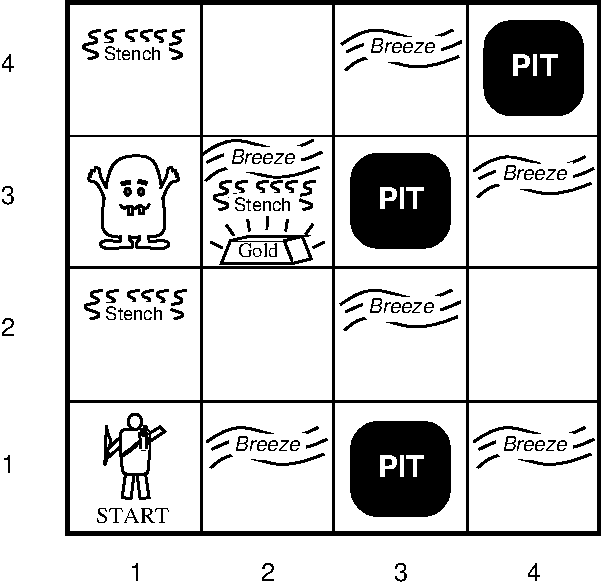
\includegraphics[height=0.8\textheight]{wumpus-world}
\end{frame}

\begin{frame}[label=wumpus-world-defined]{Wumpus World Description}
Environment:
\begin{itemize}
\item $4 \times 4$ rooms, 1 with gold, 1 with wumpus, $k$ with pits
\item Agent starts in (1,1), facing right, holding 1 arrow
\end{itemize}
Performance Measure:
\begin{itemize}
\item gold +1000, death -1000, -1 per step, -10 per arrow
\end{itemize}
\pause
Percepts:
\pause
\begin{itemize}
\item \textsc{Stench}/\textsc{Breeze} in squares adjacent to wumpus/pit
\item \textsc{Glitter} in squares with gold
\item \textsc{Bump} when running into wall
\item \textsc{Scream} when wumpus is killed by arrow
\end{itemize}
\pause
Actions:
\pause
\begin{itemize}
\item \textsc{Forward}, \textsc{TurnLeft}, \textsc{TurnRight}, \textsc{Grab}, \textsc{Shoot}
\end{itemize}
\end{frame}

\begin{frame}[label=wumpus-world-properties]{Wumpus World Properties}
\begin{description}[Deterministic?]
\item[Observable?] \uncover<2->{No, only local perception}
\item[Deterministic?] \uncover<3->{Yes, state+action determines outcome}
\item[Episodic?] \uncover<4->{No, involves a sequence of actions}
\item[Static?] \uncover<5->{Yes, pits and wumpus are stationary}
\item[Discrete?] \uncover<6->{Yes, no real-valued states or actions}
\item[Single-Agent?] \uncover<7->{Yes, wumpus takes no (real) actions}
\end{description}
\end{frame}

\begin{frame}[label=wumpus-world-example]{Exploring a Wumpus World}
\begin{center}
\begin{wumpusgrid}{4}{0.2\textheight}
\wumpusagent{1-2,5}{0}{0}
\wumpusknowledge{2-}{0}{0}{OK}
\wumpusknowledge{2-}{1}{0}{OK}
\wumpusknowledge{2-}{0}{1}{OK}
\wumpusagent{3-4}{0}{1}
\wumpuspercept{3-}{0}{1}{B}
\wumpusknowledge{4-6}{0}{2}{P?}
\wumpusknowledge{4-6}{1}{1}{P?}
\wumpusagent{6-7}{1}{0}
\wumpuspercept{6-}{1}{0}{S}
\wumpusknowledge{7-}{1}{1}{OK}
\wumpusknowledge{7-}{0}{2}{P}
\wumpusknowledge{7-}{2}{0}{W}
\wumpusagent{8-9}{1}{1}
\wumpusknowledge{9-}{2}{1}{OK}
\wumpusknowledge{9-}{1}{2}{OK}
\wumpusagent{10-}{2}{1}
\wumpuspercept{10-}{2}{1}{SG}
\end{wumpusgrid}
\end{center}
\end{frame}

\begin{frame}[label=wumpus-world-difficult]{Difficult Wumpus World Situations}
\begin{columns}
\begin{column}{0.47\textwidth}
\centering
\begin{wumpusgrid}{2}{0.18\textheight}
\wumpusagent{1-}{0}{0}
\wumpuspercept{1-}{0}{0}{S}
\wumpusknowledge{2-}{0}{1}{W?}
\wumpusknowledge{2-}{1}{0}{W?}
\end{wumpusgrid}
\begin{block}{Solution: Coercion}<3->
\textsc{Shoot} an arrow
\begin{itemize}
\item Scream \\
$\Rightarrow$ Wumpus above
\item No scream \\
$\Rightarrow$ Wumpus on right
\end{itemize}
\end{block}
\end{column}
\begin{column}{0.47\textwidth}<4->
\centering
\begin{wumpusgrid}{3}{0.18\textheight}
\wumpusagent{4-}{0}{0}
\wumpusknowledge{4-}{0}{1}{OK}
\wumpuspercept{4-}{0}{1}{B}
\wumpusknowledge{4-}{1}{0}{OK}
\wumpuspercept{4-}{1}{0}{B}
\wumpusknowledge{5-}{0}{2}{P?}
\wumpusknowledge{5-}{1}{1}{P?}
\wumpusknowledge{5-}{2}{0}{P?}
\end{wumpusgrid}
\begin{block}{Solution: Probability}<6->
% possible configurations: P_P; _P_; PP_; _PP; PPP
% configuration probabilities: (.2)(.8)(.2); (.8)(.2)(.8); (.2)(.2)(.8); (.8)(.2)(.2); (.2)(.2)(.2)
\begin{itemize}
\item 86\% pit in (2,2) % configurations 2-5
\item 31\% pit in (3,1) or (1,3) % configurations 1,3 or 1,4
\end{itemize}
\end{block}
\end{column}
\end{columns}
\end{frame}


\subsection{Logic Basics}

\begin{frame}{Logic}
	\begin{block}{Key Ideas}
		Formal language for representing information
		\begin{description}[Semantics]
			\item[Syntax] defines structure of sentences
			\item[Semantics] defines meaning of sentences
		\end{description}
	\end{block}
	\pause
	\begin{block}{Example: Arithmetic}
		\begin{description}[Semantics]
			\item[Syntax] 
				\begin{tabular}[t]{ll}
					Valid:   & $x + 2 > y$ \\
					Invalid: & $x2 + y >$
				\end{tabular}
			\item[Semantics]
				\begin{tabular}[t]{ll}
					\lefteqn{\mbox{The sentence\ } x + 2 > y \mbox{\ is true if:}} \\
					& \emph{The sum of $x$ and $2$ is greater than $y$}
				\end{tabular}
		\end{description}
	\end{block}
\end{frame}

\begin{frame}{Models}
	\begin{block}{Definitions}
		\begin{itemize}
			\item A \alert{model} is a possible state of the world
			\item If a sentence $\alpha$ is true in model $m$, \\
			      \hspace{1em} then $m$ is \alert{a model of} $\alpha$
			\item $M(\alpha)$ means \alert{all models of} $\alpha$
		\end{itemize}
	\end{block}
	\pause
	\begin{block}{Example: Arithmetic}
		Given the sentence $\alpha$ which looks like $x + 2 > y$:
		\begin{itemize}
			\pause\item Is $\{x=7, y=1\}$ a model of $\alpha$? \pause \alert{Yes}
			\pause\item Is $\{x=3, y=6\}$ a model of $\alpha$? \pause \alert{No}
		\end{itemize}
	\end{block}
\end{frame}


\subsection{Entailment}
\begin{frame}{Entailment}
\begin{columns}
\begin{column}{0.45\textwidth}
\begin{block}{Definition}
$\beta \models \alpha$ if and only if \\
\hspace{1em} $M(\beta) \subseteq M(\alpha)$\\[1em]
A sentence $\beta$ entails a sentence $\alpha$ if and only if $\alpha$ is true in all worlds where $\beta$ is true
\end{block}
\end{column}
\begin{column}{0.45\textwidth}
\begin{block}{$M(\mbox{KB}) \subseteq M(\alpha)$}
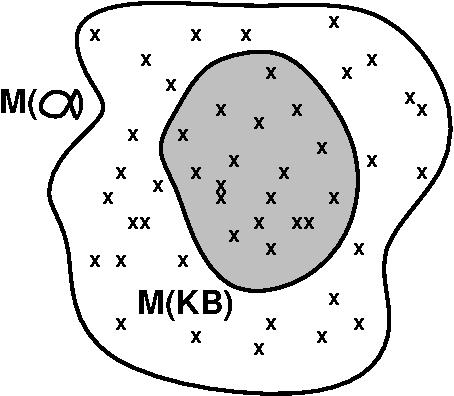
\includegraphics[width=2in]{model-inclusion}
\end{block}
\end{column}
\end{columns}
\end{frame}

\begin{frame}{Entailment Examples}
\begin{block}{Definition (Again)}
$\beta \models \alpha$ if and only if $M(\beta) \subseteq M(\alpha)$
\end{block}
\pause
\begin{itemize}[<+->]
\item $(x + y = 4) \models (4 = x + y)$
\item $(x = 0) \models (xy = 0)$
\item ``The Crimson Tide won and the Blazers won'' \\
\hspace{1em} $\models$ ``The Crimson Tide won or the Blazers won''
\end{itemize}
\end{frame}

\begin{frame}[label=wumpus-entailment]{Wumpus Entailment Example}
\begin{columns}
\begin{column}{2.5in}
\centering
\begin{wumpusgrid}{3}{0.18\textheight}
\wumpusagent{1}{0}{0}
\wumpusagent{2-}{1}{0}
\wumpuspercept{2-}{1}{0}{B}
\wumpusknowledge{3-}{0}{1}{P?}
\wumpusknowledge{3-}{1}{1}{P?}
\wumpusknowledge{3-}{2}{0}{P?}
\end{wumpusgrid}
\end{column}
\begin{column}{1.5in}
\begin{block}<4->{Models}
Number of possible models when placing pits in three squares: \\
\hspace{1em} \uncover<5->{\alert{$2^3 = 8$}}
\end{block}
\end{column}
\end{columns}
\end{frame}

\begin{frame}{Wumpus Entailment Example}
\begin{columns}
\begin{column}{0.6\textwidth}
\only<1>{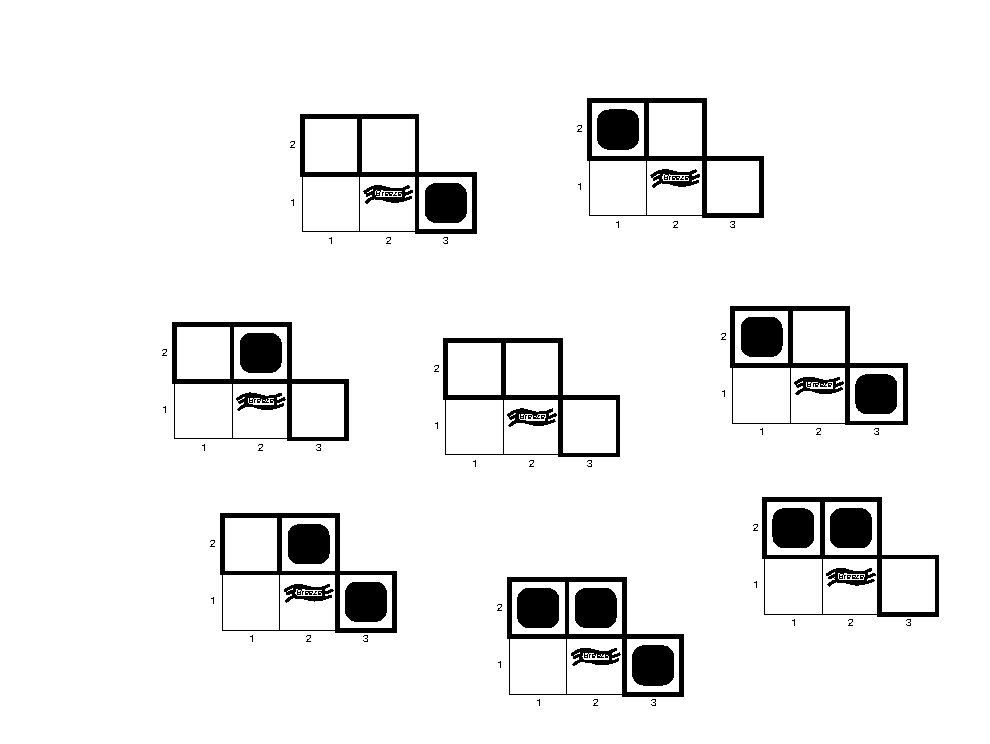
\includegraphics[width=\textwidth]{wumpus-models1}}%
\only<2>{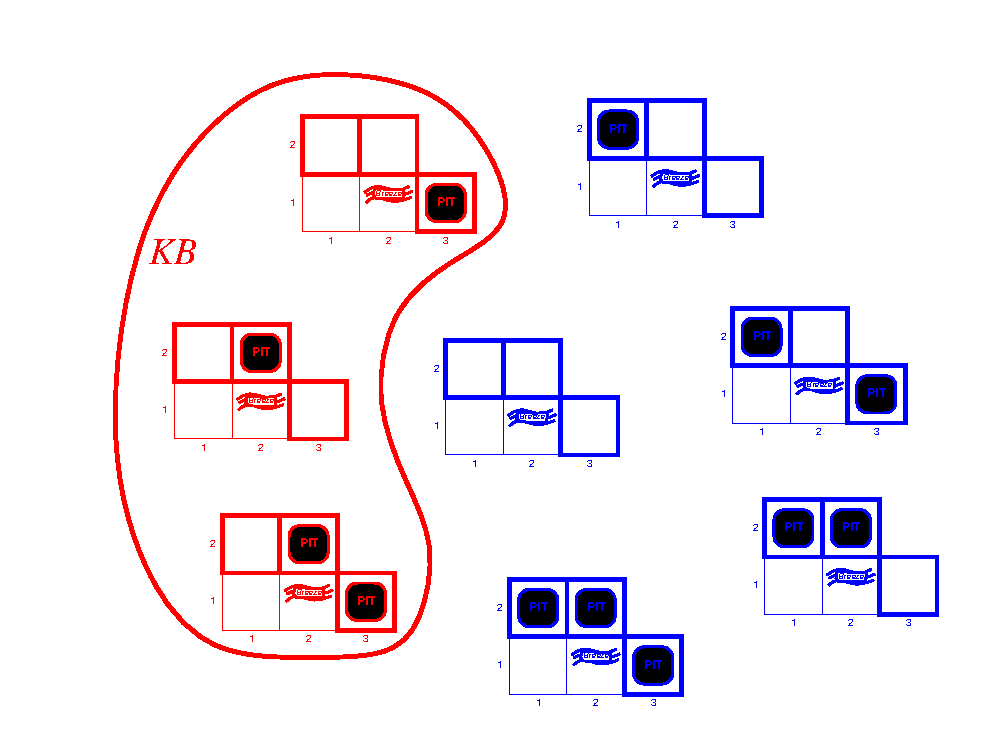
\includegraphics[width=\textwidth]{wumpus-models2}}%
\only<3-4>{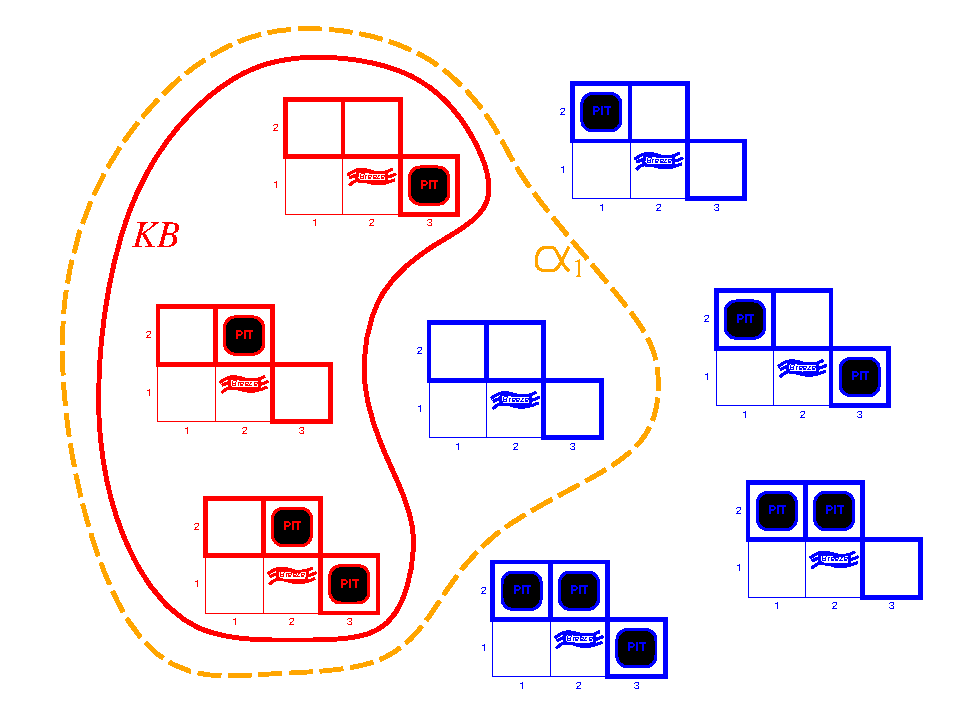
\includegraphics[width=\textwidth]{wumpus-models3}}%
\only<5-6>{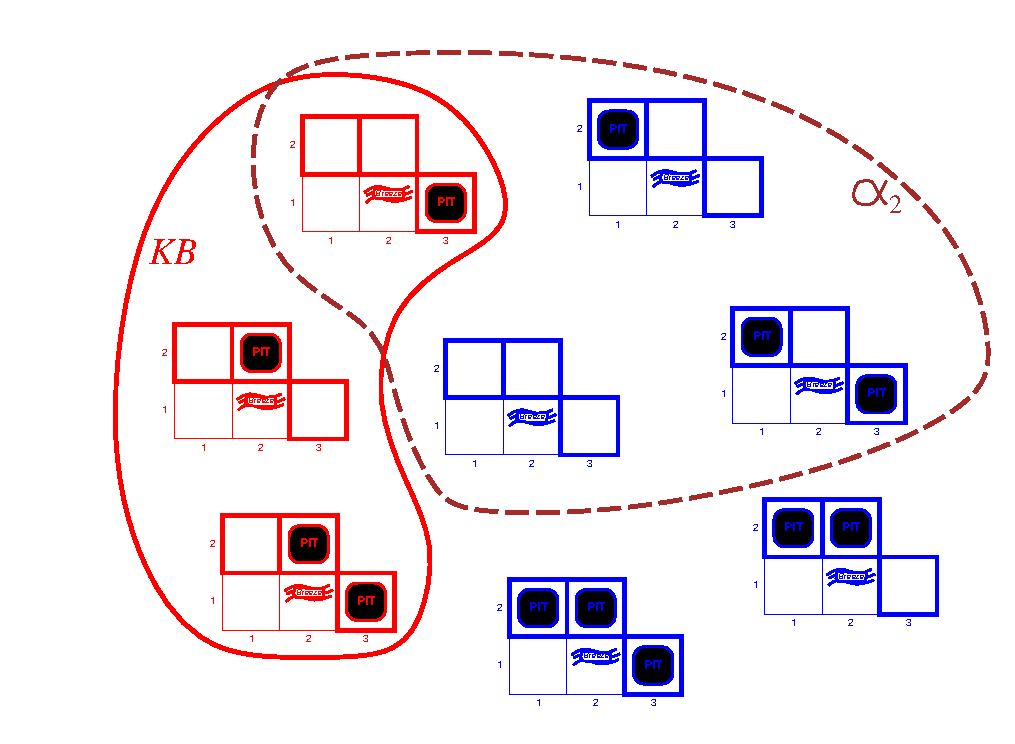
\includegraphics[width=\textwidth]{wumpus-models4}}%
\end{column}
\begin{column}{0.35\textwidth}
\uncover<2->{KB = rules + observations} \\[1em]
\uncover<3->{$\alpha_1$ = ``[1,2] is safe''} \\
\uncover<4->{$\mbox{KB} \models \alpha_1$} \\[1em]
\uncover<5->{$\alpha_2$ = ``[2,2] is safe''} \\
\uncover<6->{$\mbox{KB} \not\models \alpha_2$}
\end{column}
\end{columns}
\end{frame}


\section{Propositional Logic}
\subsection{Syntax and Semantics}

\begin{frame}{Propositional Logic Syntax}
\begin{block}{Basics}
\begin{itemize}
\item Symbols look like $P$, $Q$, $R$, etc.
\item Connectives look like:\\[0.5em]
\begin{tabular}{ll}
$\lnot$  & negation, a.k.a. ``not'' \\
$\land$  & conunction, a.k.a. ``and'' \\
$\lor$   & disjunction, a.k.a. ``or'' \\
$\limpl$ & implication, a.k.a. ``implies'' \\
$\liff$  & biconditional, a.k.a. ``equivalent''
\end{tabular}
\end{itemize}
\end{block}
\pause
\begin{block}{Examples}
\setlength{\tabcolsep}{1.5em}
\begin{tabular}{ l l l l }
$P$ &
$\lnot Q$ &
$\lnot Q \land P$ &
$R \limpl \lnot Q \land P$
\end{tabular}
\end{block}
\end{frame}

\begin{frame}{Propositional Logic Semantics}
	\begin{block}{Symbols}
		A model specifies \emph{true} or \emph{false} for each symbol \\
		\hspace{1em} E.g. $\{P=\mbox{\em true}, Q=\mbox{\em false}, R=\mbox{\em true}\}$
	\end{block}
	\pause
	\begin{block}{Connectives}
		\small
		\begin{tabular}{@{}lllll}
			$\lnot S$         & is true iff & $S$ is \emph{false} \\
			$S_1 \land S_2$   & is true iff & $S_1$ is \emph{true}            & and & $S_2$ is \emph{true} \\
			$S_1 \lor S_2$    & is true iff & $S_1$ is \emph{true}            & or  & $S_2$ is \emph{true} \\
			$S_1 \limpl S_2$  & is true iff & $S_1$ is \emph{false}           & or  & $S_2$ is \emph{true} \\
			$S_1 \liff S_2$   & is true iff & $S_1 \limpl S_2$ is \emph{true} & and & $S_2 \limpl S_1$ is \emph{true}
		\end{tabular}
	\end{block}
\end{frame}

\begin{frame}{Propositional Logic Complex Expressions}
	\begin{block}{Given}
		\begin{tabular}{lll}
			$P=\textit{true}$ & $Q=\textit{false}$ & $R=\textit{true}$ 
		\end{tabular}
	\end{block}
	\begin{block}{Evaluate}
		$P \lor R \limpl \lnot (Q \land \lnot R)$
	\end{block}
	\begin{enumerate}
		\pause\item $\textit{true} \lor \textit{true} \limpl \lnot (\textit{false} \land \lnot \textit{true})$
		\pause\item $\textit{true} \lor \textit{true} \limpl \lnot (\textit{false} \land \textit{false})$
		\pause\item $\textit{true} \lor \textit{true} \limpl \lnot \textit{false}$
		\pause\item $\textit{true} \lor \textit{true} \limpl \textit{true}$
		\pause\item $\textit{true} \limpl \textit{true}$
		\pause\item $\textit{true}$
	\end{enumerate}
\end{frame}

\begin{frame}{Implication vs. Entailment}
\begin{block}{Implication ($\alpha \limpl \beta$)}
\begin{itemize}
\item $\alpha$ is \emph{false} or $\beta$ is \emph{true}
\end{itemize}
\end{block}
\begin{block}{Entailment ($\alpha \models \beta$)}<2->
\begin{itemize}
\item In all models where $\alpha$ is true, $\beta$ is also true
\end{itemize}
\end{block}
\begin{block}{Example}<3->
\setlength{\tabcolsep}{0em}
\begin{tabular}{ l p{2em} l }
the earth is flat &
$\stackrel{\visible<3,5>{?}}{\only<3-4>{\limpl}\only<5>{\models}\only<6->{\not\models}}$ &
the moon is made of green cheese
\end{tabular}
\end{block}
\begin{block}{Relation between Implication and Entailment}<7->
$\alpha \models \beta$ if and only if $\alpha \limpl \beta$ in all models
\end{block}
\end{frame}


\subsection{Truth Tables}
\begin{frame}{Truth Tables}
	\begin{block}{Key Idea}
		\begin{itemize}
			\item Enumerate all possible values for symbols
			\item Calculate expression for each set of values
		\end{itemize}
	\end{block}
	\bigskip
	\em
	\begin{tabular}{|c|c||c|c|c|c|c|}
	\hline
	$P$   & $Q$   & $\lnot P$ & $P \land Q$ & $P \lor Q$ & $P \limpl Q$ & $P \liff Q$ \\
	\hline
	false & false & true      & false       & false      & true         & true \\
	false & true  & true      & false       & true       & true         & false \\
	true  & false & false     & false       & true       & false        & false \\
	true  & true  & false     & true        & true       & true         & true \\
	\hline
	\end{tabular}
\end{frame}

\begin{frame}{Truth Table Exercise}
\begin{block}{Problem}
Construct a truth table for $P \lor R \limpl \lnot (Q \land \lnot R)$
\end{block}
\pause
\medskip
\em
\visible<2->{
\begin{tabular}{|ccc||c|}
\hline
$P$   & $Q$   & $R$          & $P \lor R \limpl \lnot (Q \land \lnot R)$ \\
\hline
true  & true  & true  & \visible<3->{true} \\
true  & true  & false & \visible<4->{false} \\
true  & false & true  & \visible<5->{true} \\
true  & false & false & \visible<6->{true} \\
false & true  & true  & \visible<7->{true} \\
false & true  & false & \visible<8->{true} \\
false & false & true  & \visible<9->{true} \\
false & false & false & \visible<10->{true} \\
\hline
\end{tabular}
}
\end{frame}

\begin{frame}{Logical Equivalences}
	\small
	$
	\begin{array}{@{}r@{\hspace{.25em}}c@{\hspace{.25em}}l@{\hspace{.25em}}l}
	(\alpha \land \beta)                &\liff& (\beta \land \alpha)                             & \mbox{Commutativity of } \land\\
	(\alpha \lor \beta)                 &\liff& (\beta\lor \alpha)                               & \mbox{Commutativity of } \lor\\
	((\alpha \land \beta)\land \gamma)  &\liff& (\alpha\land (\beta\land \gamma))                & \mbox{Associativity of } \land\\
	((\alpha \lor \beta)\lor \gamma)    &\liff& (\alpha\lor (\beta\lor \gamma))                  & \mbox{Associativity of } \lor\\
	\lnot(\lnot \alpha)                 &\liff& \alpha                                           & \mbox{Double-negation elimination}\\
	(\alpha \limpl \beta)               &\liff& (\lnot \beta \limpl \lnot \alpha)                & \mbox{Contraposition}\\
	(\alpha \limpl \beta)               &\liff& (\lnot \alpha \lor \beta)                        & \mbox{Implication elimination}\\
	(\alpha \liff \beta)                &\liff& ((\alpha\limpl \beta)\land (\beta\limpl \alpha)) & \mbox{Biconditional elimination}\\
	\lnot(\alpha \land \beta)           &\liff& (\lnot \alpha \lor \lnot \beta)                  & \mbox{De Morgan}\\
	\lnot(\alpha \lor \beta)            &\liff& (\lnot \alpha \land \lnot \beta)                 & \mbox{De Morgan}\\
	(\alpha \land (\beta \lor \gamma))  &\liff& ((\alpha\land \beta)\lor (\alpha\land \gamma))   & \mbox{Distributivity of} \land \mbox{over } \lor\\
	(\alpha \lor (\beta \land \gamma))  &\liff& ((\alpha\lor \beta)\land (\alpha\lor \gamma))    & \mbox{Distributivity of} \lor \mbox{over } \land
	\end{array}
	$
\end{frame}


\subsection{Reasoning Patterns}

\begin{frame}{Reasoning}
\begin{block}{Key Ideas}
\begin{itemize}
\item Use logical equivalences etc. to prove things
\item No need for a truth table!
\end{itemize}
\end{block}
\pause
\begin{block}{Example}
Prove: $\lnot (P \land R \land Q)$ \\
Given: $P \land R \limpl \lnot Q$ \\
\end{block}
\bigskip
\pause
\begin{tabular}{ l @{\hspace{2em}} l }
Given & $P \land R \limpl \lnot Q$  \\
\pause Implication Elimination & \pause $\lnot (P \land R) \lor \lnot Q$ \\
\pause De Morgan & \pause $\lnot P \lor \lnot R \lor \lnot Q$ \\
\pause De Morgan & \pause $\lnot (P \land R \land Q)$ \\
\end{tabular}
\end{frame}

\begin{frame}{Additional Reasoning Patterns}
\begin{columns}[T]
\begin{column}{0.31\textwidth}
\begin{block}{Modus Ponens}
\[
\begin{array}{l}
\alpha \limpl \beta \\
\alpha \\
\hline
\beta
\end{array}
\]
\bigskip
\[
\begin{array}{l}
x > 2 \limpl x \neq 1 \\
x > 2 \\
\hline
x \neq 1
\end{array}
\]
\end{block}
\end{column}
\pause
\begin{column}{0.31\textwidth}
\begin{block}{And elimination}
\[
\begin{array}{l}
\\
\alpha \land \beta \\
\hline
\beta
\end{array}
\]
\bigskip
\[
\begin{array}{l}
\\
x = 0 \land y = 42 \\
\hline
y = 42
\end{array}
\]
\end{block}
\end{column}
\pause
\begin{column}{0.31\textwidth}
\begin{block}{Resolution}
\[
\begin{array}{l}
\alpha \lor \beta \\
\lnot\alpha \\
\hline
\beta
\end{array}
\]
\bigskip
\[
\begin{array}{l}
x = 1 \lor x = 2 \\
x \neq 1 \\
\hline
x = 2
\end{array}
\]
\end{block}
\end{column}
\end{columns}
\end{frame}

\begin{frame}[label=reasoning-exercise]{Reasoning Exercise}
\begin{columns}
\begin{column}{0.45\textwidth}
Prove: $P_{1, 3}$ \\
\bigskip
Given: \\[.2em]
$B_{1, 2}$ \\
$\lnot B_{2, 1}$ \\
$B_{1, 2} \liff (P_{1, 1} \lor P_{2, 2} \lor P_{1, 3})$ \\
$B_{2, 1} \liff (P_{1, 1} \lor P_{2, 2} \lor P_{3, 1})$ \\
\bigskip
\bigskip
\footnotesize\em
The reasoning patterns are in your book on pages 249, 250 and 252
\end{column}
\begin{column}{0.45\textwidth}
\begin{wumpusgrid}{3}{0.2\textheight}
\foreach \x in {0,...,2} \foreach \y in {0,...,2} {%
\pgfmathtruncatemacro{\xone}{1+\x}%
\pgfmathtruncatemacro{\yone}{1+\y}%
\wumpusbottom{1-}{\x}{\y}{\scriptsize (\xone,\yone)}
}
\wumpusknowledge{1-}{0}{2}{P?}
\wumpusknowledge{1-}{0}{1}{$B$}
\wumpusknowledge{1-}{1}{0}{$\neg B$}
\end{wumpusgrid}
\end{column}
\end{columns}
\end{frame}

\begin{frame}{Prove: $P_{1, 3}$}
\small
\begin{tabular}{ll}
$B_{1, 2} \liff (P_{1, 1} \lor P_{2, 2} \lor P_{1, 3})$ & Given \\
$B_{1, 2} \limpl (P_{1, 1} \lor P_{2, 2} \lor P_{1, 3})$ & Biconditional Elimination \\
$B_{1, 2}$ & Given \\
$P_{1, 1} \lor P_{2, 2} \lor P_{1, 3}$ & Modus Ponens \\
\hline
$B_{2, 1} \liff (P_{1, 1} \lor P_{2, 2} \lor P_{3, 1})$ & Given \\
$(P_{1, 1} \lor P_{2, 2} \lor P_{3, 1}) \limpl B_{2, 1}$ & Biconditional Elimination \\
$\lnot B_{2, 1} \limpl \lnot(P_{1, 1} \lor P_{2, 2} \lor P_{3, 1})$ & Contraposition \\
$\lnot B_{2, 1}$ & Given \\
$\lnot(P_{1, 1} \lor P_{2, 2} \lor P_{3, 1})$ & Modus Ponens \\
$\lnot P_{1, 1} \land \lnot P_{2, 2} \land \lnot P_{3, 1}$ & De Morgan \\
\hline
$\lnot P_{1, 1}$ & And-Elimination \\
$P_{2, 2} \lor P_{1, 3}$ & Resolution \\
$\lnot P_{2, 2}$ & And-Elimination \\
$P_{1, 3}$ & Resolution \\
\end{tabular}
\end{frame}


\section{Inference Algorithms}
\begin{frame}{Inference Algorithms}
	\begin{block}{Definition: Derives}
		Procedure $i$ \alert{derives} $\beta$ from $\alpha$ ($\alpha \vdash_i \beta$) if:\\
		\hspace{1em} when given $\alpha$, procedure $i$ is able to conclude $\beta$
	\end{block}
	\pause
	\begin{block}{Definition: Soundness}
		Procedure $i$ is \alert{sound} if:\\
		\hspace{1em} whenever $\alpha \vdash_i \beta$ it is also true that $\alpha \models \beta$
	\end{block}
	\pause
	\begin{block}{Definition: Completeness}
		Procedure $i$ is \alert{complete} if:\\
		\hspace{1em} whenever $\alpha \models \beta$ it is also true that $\alpha \vdash_i \beta$
	\end{block}
\end{frame}


\subsection{Truth Tables}
\begin{frame}{Inference by Truth Table}
	\small
	\begin{columns}[T]
		\begin{column}{.8in}
			Prove: \\[.2em]
			$
			\begin{array}{l}
				\lnot P_{1,2}
			\end{array}
			$
		\end{column}
		\begin{column}{3.4in}
			Given: \\[.2em]
			\small
			$
			\begin{array}{llll}
			R_1: & \lnot P_{1,1}                                     & R_4: & \lnot B_{1,1} \\
			R_2: & B_{1,1} \liff (P_{1,2} \lor P_{2,1})              & R_5: & B_{2,1}\\
			R_3: & B_{2,1} \liff (P_{1,1} \lor P_{2,2} \lor P_{3,1})
			\end{array}
			$
		\end{column}
	\end{columns}
	\pause
	
	\medskip	
	\em\scriptsize
	\begin{tabular}{
		|@{\hspace{.3em}}c@{\hspace{.4em}}
		|@{\hspace{.3em}}c@{\hspace{.4em}}
		|@{\hspace{.3em}}c@{\hspace{.4em}}
		|@{\hspace{.3em}}c@{\hspace{.4em}}
		|@{\hspace{.3em}}c@{\hspace{.4em}}
		|@{\hspace{.3em}}c@{\hspace{.4em}}
		|@{\hspace{.3em}}c@{\hspace{.4em}}
		||@{\hspace{.3em}}c@{\hspace{.4em}}
		|@{\hspace{.3em}}c@{\hspace{.4em}}
		|@{\hspace{.3em}}c@{\hspace{.4em}}
		|@{\hspace{.3em}}c@{\hspace{.4em}}
		|@{\hspace{.3em}}c@{\hspace{.4em}}
		||@{\hspace{.3em}}c@{\hspace{.4em}}
		|}
		\hline
		$B_{1,1}$ & $B_{2,1}$ & $P_{1,1}$ & $P_{1,2}$ & $P_{2,1}$ & $P_{2,2}$ & $P_{3,1}$ & $R_{1}$ & $R_{2}$ & $R_{3}$ & $R_{4}$ & $R_{5}$ & KB \\
		\hline
		false   & false   & false   & false   & false   & false   & false   & true  & true  & true  & true  & false & false \\
		false   & false   & false   & false   & false   & false   & true    & true  & true  & false & true  & false & false \\
		\vdots  & \vdots  & \vdots  & \vdots  & \vdots  & \vdots  & \vdots  & \vdots& \vdots& \vdots& \vdots& \vdots& \vdots \\
		false   & true    & false   & false   & false   & false   & false   & true  & true  & false & true  & true  & false \\
		\hline
		false   & true    & false   & \alert<5>{false}   & false   & false   & true    & \alert<3>{true}  & \alert<3>{true}  & \alert<3>{true}  & \alert<3>{true}  & \alert<3>{true}  & \alert<4->{true} \\
		false   & true    & false   & \alert<5>{false}   & false   & true    & false   & \alert<3>{true}  & \alert<3>{true}  & \alert<3>{true}  & \alert<3>{true}  & \alert<3>{true}  & \alert<4->{true} \\
		false   & true    & false   & \alert<5>{false}   & false   & true    & true    & \alert<3>{true}  & \alert<3>{true}  & \alert<3>{true}  & \alert<3>{true}  & \alert<3>{true}  & \alert<4->{true} \\
		\hline
		false   & true    & false   & false   & true    & false   & false   & true  & false & false & true  & true  & false \\
		\vdots  & \vdots  & \vdots  & \vdots  & \vdots  & \vdots  & \vdots  & \vdots& \vdots& \vdots& \vdots& \vdots& \vdots \\
		true    & true    & true    & true    & true    & true    & true    & false & true  & true  & false & true  & false \\
		\hline
	\end{tabular}
\end{frame}
\begin{frame}[fragile]{Truth Table Inference Code}
	\begin{semiverbatim}\scriptsize\bfseries
		\keyword{def} \defn{truth_table_entails}(knowledge_base, query):\pause
		    \cmnt{# check all assignments of knowledge base and query symbols:}
		    \cmnt{# if the knowledge base is true the query should be true}
		    symbols = set.union(knowledge_base.symbols, query.symbols)
		    \keyword{return} all(
		        query.is_true_for(assignment)
		        \keyword{for} assignment \keyword{in} all_models(symbols)
		        \keyword{if} knowledge_base.is_true_for(assignment))
		
		\pause\keyword{def} \defn{all_models}(symbols):
		    \pause\cmnt{# base case: no symbols, generate an empty assignment}
		    \keyword{if} \keyword{not} symbols:
		        \keyword{yield} \{\}
		    \pause\cmnt{# recursive case: assign to the first symbol and recurse}
		    \keyword{else}:
		        first, rest = symbols[0], symbols[1:]
		        \keyword{for} assignment \keyword{in} all_models(rest):
		            \keyword{for} value \keyword{in} [True, False]:
		                assignment[first] = value
		                \keyword{yield} assignment	
	\end{semiverbatim}
\end{frame}

\begin{frame}{Truth Table Inference Properties}
\begin{block}{Definitions (Again)}
\begin{description}
\item[Sound] if $\alpha \vdash_i \beta$ then $\alpha \models \beta$
\item[Complete] if $\alpha \models \beta$ then $\alpha \vdash_i \beta$
\end{description}
\end{block}
\begin{block}{Truth Table Inference Properties}
\begin{description}[Complete?]
\item[Sound?] \uncover<2->{Yes, directly implements entailment definition}
\item[Complete?] \uncover<3->{Yes, explores all possibilities}
\item[Time?] \uncover<4->{Given $n$ symbols, takes $O(2^n)$}
\end{description}
\end{block}
\end{frame}


\subsection{Chaining}

\begin{frame}{Forward and Backward Chaining}
\begin{block}{Key Idea}
Inference is easier if all statements are \alert{Horn Clauses}: \\
\hspace{1em} $P_1 \land \ldots \land P_n \limpl Q$ \\
\end{block}%
\begin{columns}[t]<2->
\begin{column}{0.3\textwidth}
Given: \\[.2em]
$
\begin{array}{l}
B \land L \limpl M \\
A \land B \limpl L \\
A \\
B
\end{array}
$
\end{column}
\begin{column}{0.65\textwidth}
Prove $M$: \\[.2em]
$
\begin{array}{ll}
\visible<3->{A \\
B \\
A \land B \limpl L \\
\hline}
\visible<4->{L & \mbox{by Modus Ponens}} \\
\visible<5->{B \\
B \land L \limpl M \\
\hline}
\visible<6->{M & \mbox{by Modus Ponens}}
\end{array}
$
\end{column}
\end{columns}
\end{frame}

\begin{frame}[fragile]{Forward Chaining Code}
	\begin{semiverbatim}\bfseries\scriptsize
		\keyword{def} \defn{forward_chaining_entails}(knowledge_base, query):
		    \pause\cmnt{# count the symbols in the premise of each clause}
		    counts = \{\}
		    \keyword{for} clause \keyword{in} knowledge_base.get_clauses():
		        counts[clause] = len(clause.premise)
		    \pause\cmnt{# start with known symbols and search for non-inferred}
		    inferred = set()
		    agenda = knowledge_base.get_true_symbols()
		    \keyword{while} agenda:
		        symbol = agenda.pop()
		        \pause\cmnt{# if the query was on the agenda, it is known to be true}
		        \keyword{if} symbol == query:
		            \keyword{return} \keyword{True}
		        \pause\cmnt{# do not repeat symbols that have already been checked}
		        \keyword{if} symbol \keyword{not in} inferred:
		            inferred.add(symbol)
		            \pause\cmnt{# update counts and infer conclusions when possible}
		            \keyword{for} clause \keyword{in} knowledge_base.get_clauses():
		                \keyword{if} symbol \keyword{in} clause.premise:
		                    counts[clause] -= 1
		                    \keyword{if} counts[clause] == 0:
		                        agenda.append(clause.head)
		    \pause\keyword{return} \keyword{False}
	\end{semiverbatim}
\end{frame}

\begin{frame}[label=forward-chaining-example]{Forward Chaining Example}
\begin{columns}
\begin{column}{0.3\textwidth}
\large
\hspace{2em} $
\begin{array}{l}
P \limpl Q \\
L \land M \limpl P \\
B \land L \limpl M \\
A \land P \limpl L \\
A \land B \limpl L \\
A \\
B
\end{array}
$
\end{column}
\begin{column}{0.65\textwidth}
\small
\begin{tikzpicture}[
  every edge/.style={draw,-latex},
  every label/.style={color=red},
  symbol/.style={draw,circle},
  clause/.style={draw}]
\node[symbol,red edge on={2-4},red fill on={3-4}] at (0, 0) (A) {$A$};
\node[symbol,red edge on={2-7},red fill on={5-7}] at (5, 0) (B) {$B$};
\node[symbol,red edge on={7-10,16-17},red fill on={8-10,17}] at (2.5, 2) (L) {$L$};
\node[symbol,red edge on={10-13},red fill on={11-13}] at (5, 4) (M) {$M$};
\node[symbol,red edge on={13-16},red fill on={14-16}] at (0, 4) (P) {$P$};
\node[symbol,red edge on={16-,18-},red fill on={18-}] at (2.5, 6) (Q) {$Q$};
\node[clause,label=30:{\only<1-3>{2}\only<4-5>{1}\only<6->{0}}] at (2.5, 0) (ABL) {$A \land B \limpl L$};
\node[clause,label=30:{\only<1-3>{2}\only<4-14>{1}\only<15->{0}}] at (0, 2) (APL) {$A \land P \limpl L$};
\node[clause,label=30:{\only<1-5>{2}\only<6-8>{1}\only<9->{0}}] at (5, 2) (BLM) {$B \land L \limpl M$};
\node[clause,label=30:{\only<1-8>{2}\only<9-11>{1}\only<12->{0}}] at (2.5, 4) (LMP) {$L \land M \limpl P$};
\node[clause,label=30:{\only<1-14>{1}\only<15->{0}}] at (0, 6) (PQ) {$P \limpl Q$};
\path (A) edge (ABL);
\path (B) edge (ABL);
\path (ABL) edge (L);
\path (A) edge (APL);
\path (P) edge (APL);
\path (APL) edge (L);
\path (B) edge (BLM);
\path (L) edge (BLM);
\path (BLM) edge (M);
\path (L) edge (LMP);
\path (M) edge (LMP);
\path (LMP) edge (P);
\path (P) edge (PQ);
\path (PQ) edge (Q);
\end{tikzpicture}
\end{column}
\end{columns}
\end{frame}

\begin{frame}{Forward Chaining Properties}
\begin{block}{Properties}
\begin{description}[Complete?]
\item[Sound?] \uncover<2->{Yes, uses Modus Ponens}
\item[Complete?] \uncover<3->{Yes (more on this in a moment)}
\item[Time?] \uncover<4->{$O(n)$ given $n$ statements in KB}
\end{description}
\end{block}
\begin{block}{Reminder}<5->
\begin{itemize}
\item Requires Horn Clauses
\item Won't work with Propositional logic in general
\end{itemize}
\end{block}
\end{frame}

\begin{frame}{Forward Chaining Completeness}
	\begin{block}{Prove: If $\textit{KB} \models Q$ then $\textit{KB} \vdash_{\textit{\scriptsize forward-chaining}} Q$}
		\begin{enumerate}
			\item<2-> $\textit{KB} \models Q$, so $Q$ is \emph{true} in every model of \emph{KB}
			\item<4-> Final \texttt{inferred} set is a model of \emph{KB}
			\item<4-> So $Q$ is true in the \texttt{inferred} model
			\item<4-> So $\textit{KB} \vdash_{\textit{\scriptsize forward-chaining}} Q$
		\end{enumerate}
	\end{block}
	\begin{block}<3->{Prove: The final \texttt{inferred} set is a model of $\textit{KB}$}
		\begin{enumerate}
			\item Assume not, i.e. $P_1 \land \ldots \land P_n \limpl Q$ is \emph{false}
			\item So $P_1 \land \ldots \land P_n$ is \emph{true} and $Q$ is \emph{false} (= not inferred)
			\item But then $Q$ should have been inferred!
			\item So \texttt{inferred} must be a model of KB
		\end{enumerate}
	\end{block}
\end{frame}

\begin{frame}[label=backward-chaining]{Backward Chaining}
\begin{block}{Key Idea: Recursion}
\begin{itemize}
\item Start by trying to prove query $Q$
\item If not \emph{true}, try to prove $P_1 \land \ldots \land P_n \limpl Q$ (recurse)
\end{itemize}
\end{block}
\begin{columns}
\begin{column}{0.55\textwidth}
\small
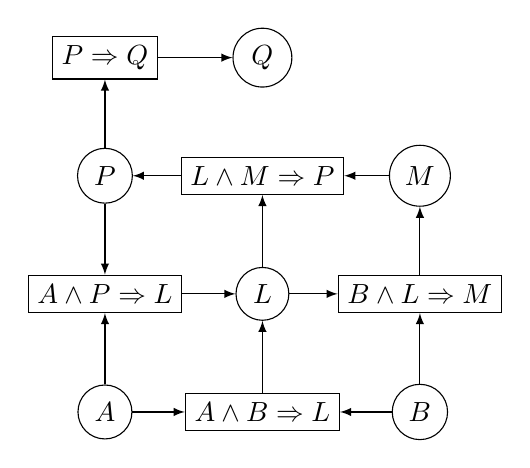
\begin{tikzpicture}[
  every edge/.style={draw,-latex},
  every label/.style={color=red},
  symbol/.style={draw,circle},
  clause/.style={draw}]
\node[symbol,red edge fill on={2-}] at (0, 0) (A) {$A$};
\node[symbol,red edge fill on={2-}] at (4, 0) (B) {$B$};
\node[symbol,blue edge on={6-11},blue fill on={7-11},red edge fill on={12-}] at (2, 1.5) (L) {$L$};
\node[symbol,blue edge on={6-14},blue fill on={13-14},red edge fill on={15-}] at (4, 3) (M) {$M$};
\node[symbol,blue edge on={4-16},blue fill on={5-16},red edge fill on={17-}] at (0, 3) (P) {$P$};
\node[symbol,blue edge on={2-18},blue fill on={3-18},red edge fill on={19-}] at (2, 4.5) (Q) {$Q$};
\node[clause,blue edge on={7-},blue fill on={10},red edge fill on={11-}] at (2, 0) (ABL) {$A \land B \limpl L$};
\node[clause,blue edge on={7-8},blue fill on={8}] at (0, 1.5) (APL) {$A \land P \limpl L$};
\node[clause,blue edge on={13},red edge fill on={14-}] at (4, 1.5) (BLM) {$B \land L \limpl M$};
\node[clause,blue edge on={5-15},blue fill on={6-15},red edge fill on={16-}] at (2, 3) (LMP) {$L \land M \limpl P$};
\node[clause,blue edge on={3-17},blue fill on={4-17},red edge fill on={18-}] at (0, 4.5) (PQ) {$P \limpl Q$};
\path (A) edge (ABL);
\path (B) edge (ABL);
\path (ABL) edge (L);
\path (A) edge (APL);
\path (P) edge (APL);
\path (APL) edge (L);
\path (B) edge (BLM);
\path (L) edge (BLM);
\path (BLM) edge (M);
\path (L) edge (LMP);
\path (M) edge (LMP);
\path (LMP) edge (P);
\path (P) edge (PQ);
\path (PQ) edge (Q);
\end{tikzpicture}
\end{column}
\begin{column}{0.4\textwidth}<20->
\begin{block}{Properties}
\begin{description}[Complete?]
\item[Sound?] Yes
\item[Complete?] Yes
\item[Time?] $O(n)$ and often less
\end{description}
\end{block}
\end{column}
\end{columns}
\end{frame}

\subsection{Resolution}

\begin{frame}{Resolution (Again)}
	\begin{block}{Example}
		$
		\begin{array}{l}
		\lnot \textit{IsSnowing} \lor \textit{IsCold} \\
		\lnot \textit{IsCold} \lor \textit{WearCoat} \\
		\hline
		\lnot \textit{IsSnowing} \lor \textit{WearCoat}
		\end{array}
		$
	\end{block}
	\begin{block}{Intuition}
		\begin{itemize}
			\item If \textit{IsCold} is \emph{true}, then \textit{WearCoat} must be \emph{true}
			\item If \textit{IsCold} is \emph{false}, then \textit{IsSnowing} must be \emph{false}
			\item So either \textit{IsSnowing} is \emph{false} or \textit{WearCoat} is \emph{true}
		\end{itemize}
	\end{block}
\end{frame}
\begin{frame}{Resolution}
	\begin{block}{Resolution Definition}
	\small
	$
	\begin{array}{l}
		P_1 \lor \ldots \lor P_n \\[.2em]
		Q_1 \lor \ldots \lor Q_m \\[.2em]
		P_i = \lnot Q_j \\[.2em]
		\hline
		\\[-.8em]
		P_1 \!\lor\! \ldots \!\lor\! P_{i-1} \!\lor\! P_{i+1} \!\lor\! \ldots \!\lor\! P_n
		\lor
		Q_1 \!\lor\! \ldots \!\lor\! Q_{j-1} \!\lor\! Q_{j+1} \!\lor\! \ldots \!\lor\! Q_m
	\end{array}
	$
	\end{block}
	\begin{block}{Inference by Resolution}
		\begin{itemize}
			\item Simplify all statements to use only $\land$, $\lor$ and $\lnot$
			\item Assume $\textit{KB} \land \lnot\alpha$ (a.k.a $\lnot (\textit{KB} \limpl \alpha)$)
			\item Apply resolution until \emph{false} is concluded
		\end{itemize}
	\end{block}
\end{frame}

\begin{frame}[label=resolution-example]{Resolution Example}
\begin{columns}[t]
\begin{column}{1.5in}
Prove: $A$ \\[1em]
Given: \\
\begin{tabular}{ll}
$R_1\!\!:$ & $A \lor B$ \\
$R_2\!\!:$ & $C \lor \lnot B$ \\
$R_3\!\!:$ & $A \lor \lnot C$ \\
\end{tabular}
\end{column}
\begin{column}{2.5in}
Proof: \\[1em]
\begin{tabular}{lll}
\visible<2->{$R_4\!\!:$    & $\lnot A$         & Assumed} \\
\visible<3->{$R_5\!\!:$    & $B$               & $R_1$, $R_4$} \\
\visible<4->{$R_6\!\!:$    & $\lnot C$         & $R_3$, $R_4$} \\
\visible<5->{$R_7\!\!:$    & $\lnot B$         & $R_2$, $R_6$} \\
\visible<6->{$R_8\!\!:$    & \emph{false}      & $R_5$, $R_7$} \\
\end{tabular}
\end{column}
\end{columns}
\end{frame}

\begin{frame}{Conjunctive Normal Form}
	\begin{block}{Goal: Conjunction of Disjunctions of Literals}
		$(P_1 \lor \ldots \lor P_n) \land (Q_1 \lor \ldots \lor Q_m) \land \ldots$
	\end{block}
	\begin{block}{Procedure}
		\begin{enumerate}
			\item Replace $\alpha \liff \beta$ with $(\alpha\limpl \beta)\land (\beta\limpl \alpha)$
			\item Replace $\alpha \limpl \beta$ with $\lnot\alpha \lor \beta$
			\item Move $\lnot$ inward with De Morgan and Double Negation
			\item Apply Distributivity of $\lor$ over $\land$
		\end{enumerate}
	\end{block}
\end{frame}
\begin{frame}{Conjunctive Normal Form Example}
	\hspace{2em} $B_{1,1} \liff (P_{1,2} \lor P_{2,1})$
	\begin{enumerate}
		\pause\vspace{.5em}\item
			Replace $\alpha \liff \beta$ with $(\alpha \limpl \beta)\land (\beta\limpl \alpha)$ \\
			\pause
			$(B_{1,1} \limpl (P_{1,2} \lor P_{2,1})) \land ((P_{1,2} \lor P_{2,1}) \limpl B_{1,1})$
		
		\pause\vspace{.5em}\item
			Replace $\alpha \limpl \beta$ with $\lnot\alpha \lor \beta$ \\
			\pause
			$(\lnot B_{1,1} \lor P_{1,2} \lor P_{2,1}) \land (\lnot(P_{1,2} \lor P_{2,1}) \lor B_{1,1})$
		
		\pause\vspace{.5em}\item
			Move $\lnot$ inward with De Morgan and Double Negation \\
			\pause
			$(\lnot B_{1,1} \lor P_{1,2} \lor P_{2,1}) \land ((\lnot P_{1,2} \land \lnot P_{2,1}) \lor B_{1,1})$
		
		\pause\vspace{.5em}\item
			Apply Distributivity of $\lor$ over $\land$ \\
			\pause
			$(\lnot B_{1,1} \lor P_{1,2} \lor P_{2,1}) \land (\lnot P_{1,2} \lor B_{1,1}) \land (\lnot P_{2,1} \lor B_{1,1})$
	\end{enumerate}
\end{frame}

\begin{frame}[label=resolution-exercise]{Resolution Exercise}
\begin{columns}[T]
\begin{column}{0.45\textwidth}
Prove using Resolution:\\[.2em]
$P_{1, 3}$\\
\bigskip
Given: \\[.2em]
$B_{1, 2}$ \\
$\lnot B_{2, 1}$ \\
$B_{1, 2} \liff (P_{1, 1} \lor P_{2, 2} \lor P_{1, 3})$ \\
$B_{2, 1} \liff (P_{1, 1} \lor P_{2, 2} \lor P_{3, 1})$
\end{column}
\begin{column}{0.45\textwidth}
\begin{wumpusgrid}{3}{0.2\textheight}
\foreach \x in {0,...,2} \foreach \y in {0,...,2} {%
\pgfmathtruncatemacro{\xone}{1+\x}%
\pgfmathtruncatemacro{\yone}{1+\y}%
\wumpusbottom{1-}{\x}{\y}{\scriptsize (\xone,\yone)}
}
\wumpusknowledge{1-}{0}{2}{P?}
\wumpusknowledge{1-}{0}{1}{$B$}
\wumpusknowledge{1-}{1}{0}{$\neg B$}
\end{wumpusgrid}
\end{column}
\end{columns}
\end{frame}

\begin{frame}[label=resolution-exercise-solution]{Prove: $P_{1, 3}$}
	\begin{columns}[t]
		\begin{column}{0.45\textwidth}
			After conversion to CNF: \\[.5em]
			\small
			\begin{tabular}{@{}l@{\hspace{.2em}}l@{}}
				$R_1\!\!:$ & $B_{1, 2}$ \\
				$R_2\!\!:$ & $\lnot B_{2, 1}$ \\
				$R_3\!\!:$ & $\lnot B_{1, 2} \!\lor\! P_{1, 1} \!\lor\! P_{2, 2} \!\lor\! P_{1, 3}$ \\
				$R_4\!\!:$ & $\lnot P_{1, 1} \!\lor\! B_{1, 2}$ \\
				$R_5\!\!:$ & $\lnot P_{2, 2} \!\lor\! B_{1, 2}$ \\
				$R_6\!\!:$ & $\lnot P_{1, 3} \!\lor\! B_{1, 2}$ \\
				$R_7\!\!:$ & $\lnot B_{2, 1} \!\lor\! P_{1, 1} \!\lor\! P_{2, 2} \!\lor\! P_{3, 1}$ \\
				$R_8\!\!:$ & $\lnot P_{1, 1} \!\lor\! B_{2, 1}$ \\
				$R_9\!\!:$ & $\lnot P_{2, 2} \!\lor\! B_{2, 1}$ \\
				$R_{10}\!\!:$ & $\lnot P_{3, 1} \!\lor\! B_{2, 1}$ \\
			\end{tabular}
		\end{column}
		\begin{column}{0.52\textwidth}
			Using resolution: \\[.5em]
			\small
			\begin{tabular}{@{}l@{\hspace{.2em}}ll@{}}
				$R_{11}\!\!:$ & $\lnot P_{1, 3}$                                     & Assumed \\
				$R_{12}\!\!:$ & $\lnot P_{1, 1}$                                     & $R_{2}$  + $R_{8}$ \\
				$R_{13}\!\!:$ & $\lnot P_{2, 2}$                                     & $R_{2}$  + $R_{9}$ \\
				$R_{14}\!\!:$ & $\lnot B_{1, 2} \!\lor\! P_{1, 1} \!\lor\! P_{2, 2}$ & $R_{11}$ + $R_{3}$ \\
				$R_{15}\!\!:$ & $P_{1, 1} \!\lor\! P_{2, 2}$                         & $R_{14}$ + $R_{1}$  \\
				$R_{16}\!\!:$ & $P_{2, 2}$                                           & $R_{15}$ + $R_{12}$ \\
				$R_{17}\!\!:$ & \emph{false}                                         & $R_{16}$ + $R_{13}$\\
			\end{tabular}
		\end{column}
	\end{columns}
\end{frame}

\begin{frame}{Resolution Properties}
\begin{block}{Properties}
\begin{description}[Complete?]
\item[Sound?] \uncover<2->{Yes, uses Resolution}
\item[Complete?] \uncover<3->{Yes}
\item[Time?] \uncover<4->{Worst case exponential in \# of symbols}
\end{description}
\end{block}
\begin{block}{Notes}<5->
\begin{itemize}
\item Works for Propositional logic in general
\item Not just Horn Clauses!
\end{itemize}
\end{block}
\end{frame}

\subsection{WalkSAT}

\begin{frame}{WalkSAT}
\begin{block}{Key Ideas}
\begin{itemize}
\item Treat satisfiability checking as local search
\item On each iteration flip a symbol's value
\item Choice of symbol to flip is sometimes random, sometimes by \textsc{Min-Conflicts}
\item Quit after a certain number of steps
\end{itemize}
\end{block}
\begin{block}{Properties}
\begin{description}[Complete?]
\item[Sound?] \uncover<2->{Yes, only returns when KB is \emph{true}}
\item[Complete?] \uncover<3->{No, could stop early}
\item[Time?] \uncover<4->{Can be quite fast}
\end{description}
\end{block}
\end{frame}

\begin{frame}{WalkSAT Performance}
	\begin{columns}
		\begin{column}{3.2in}
			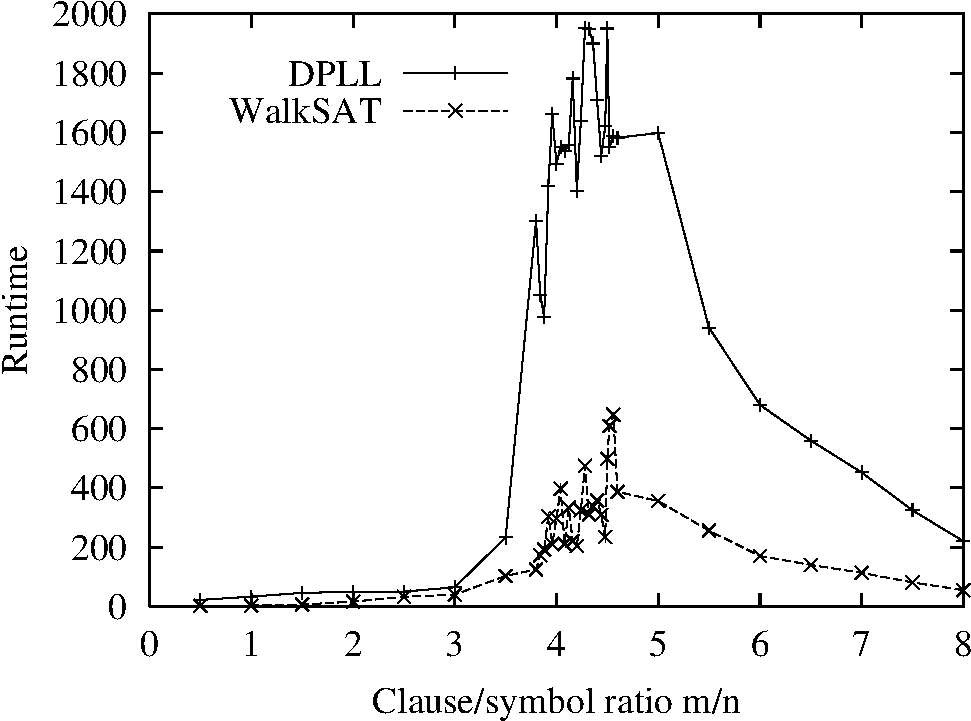
\includegraphics[width=3.2in]{random-3sat-performance}
		\end{column}
		\begin{column}{1in}
			\keyword{DPLL} \\
			Truth table entailment + heuristics and pruning
		\end{column}
	\end{columns}
\end{frame}

\part{Key Points}
\begin{frame}{Key Points}
	\begin{block}{Propositional Logic}
		\begin{itemize}
			\item Symbols: $P$, $Q$, $R$, $\ldots$
			\item Connectives: $\land$, $\lor$, $\lnot$, $\limpl$, $\liff$, 
			\item Entailment: $\alpha \models \beta$ iff $\alpha \limpl \beta$ in all worlds
		\end{itemize}
	\end{block}
	\begin{block}{Inference}
		\begin{itemize}
			\item Enumerate all models through truth tables
			\item Forward/Backward chaining with Horn clauses
			\item Resolution using conjunctive normal form
			\item Local search, e.g. \textsc{WalkSAT}
		\end{itemize}
	\end{block}
\end{frame}


\end{document}


